\documentclass[tikz,border=2pt]{standalone}
\usepackage{amsmath,amssymb}
\usepackage{pgfplots}
\pgfplotsset{compat=1.18}
\usetikzlibrary{arrows.meta}
\begin{document}
% T_0 ~ U(0,100): S_0(y) = 1 - y/100. Given survival to 60, P(T_60 > t) = S_0(60+t)/S_0(60) = (40-t)/40,
% drawn against attained age 60+t; at age 70 it is 0.3/0.4 = 0.75.
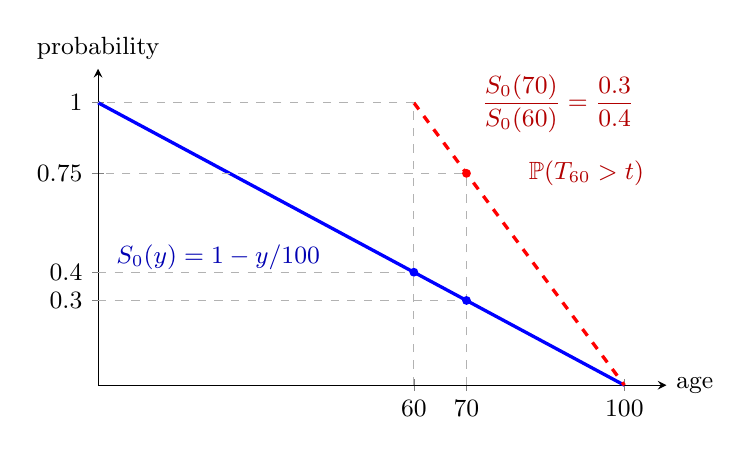
\begin{tikzpicture}[font=\small, >={Latex[length=2mm]}]
  \begin{axis}[
    axis lines=left, xmin=0, xmax=108, ymin=0, ymax=1.12,
    xtick={60,70,100}, ytick={0.3,0.4,0.75,1},
    yticklabels={$0.3$,$0.4$,$0.75$,$1$},
    xlabel={age}, ylabel={probability},
    xlabel style={at={(axis description cs:1,0)}, anchor=west},
    ylabel style={rotate=-90, at={(axis description cs:0,1)}, anchor=south},
    width=8.8cm, height=5.6cm, clip=false]
    \addplot[blue, very thick, domain=0:100] {1-x/100};
    \addplot[red, very thick, dashed, domain=60:100] {(100-x)/40};
    \draw[gray!60, thin, dashed] (axis cs:60,0) -- (axis cs:60,1) -- (axis cs:0,1);
    \draw[gray!60, thin, dashed] (axis cs:70,0) -- (axis cs:70,0.75) -- (axis cs:0,0.75);
    \draw[gray!60, thin, dashed] (axis cs:0,0.4) -- (axis cs:60,0.4);
    \draw[gray!60, thin, dashed] (axis cs:0,0.3) -- (axis cs:70,0.3);
    \fill[blue] (axis cs:60,0.4) circle (1.6pt);
    \fill[blue] (axis cs:70,0.3) circle (1.6pt);
    \fill[red] (axis cs:70,0.75) circle (1.6pt);
    \node[blue!70!black, anchor=north east] at (axis cs:44,0.53) {$S_0(y)=1-y/100$};
    \node[red!70!black, anchor=west] at (axis cs:80,0.75) {$\mathbb P(T_{60}>t)$};
    \node[red!70!black, anchor=south west] at (axis cs:71,0.86) {$\dfrac{S_0(70)}{S_0(60)}=\dfrac{0.3}{0.4}$};
  \end{axis}
\end{tikzpicture}
\end{document}
